\subsection{Effects of Different Hyperparameters}
\label{sec:subtask3}

In this task, we firstly choose $9$ different settings to study the effects of different hyperparameters on the transformer model, which are shown in \cref{fig:different_settings}.
To further study the impact of weight decay, we plot the accuracy curves for $8$ different weight decay values, which is shown in \cref{fig:different weight_decay}.
With a parameter setting of $p=97$, we employ a step budget of $10^5$, a decision inspired by the original paper's use. 
Similarly, the training accuracies raise up to $99\%$ within $10^3$ steps in most experiments, but the validation accuracies differ from each other.

\begin{figure}[!ht]
    \centering
    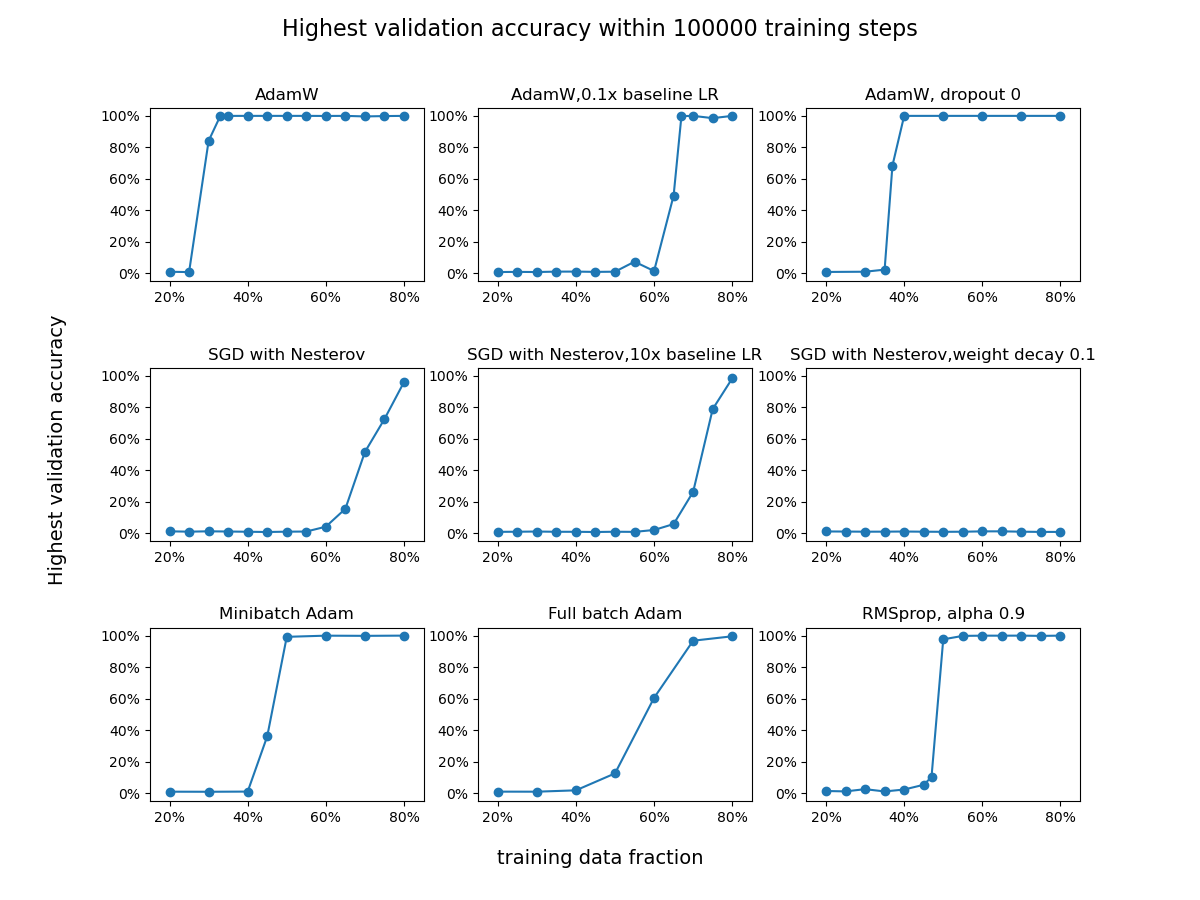
\includegraphics[width=0.9\textwidth]{fig/different_settings/different_settings.png}
    \caption{Grokking phenomenon for different settings}
    \label{fig:different_settings}
\end{figure}
\begin{figure}[!ht]
    \centering
    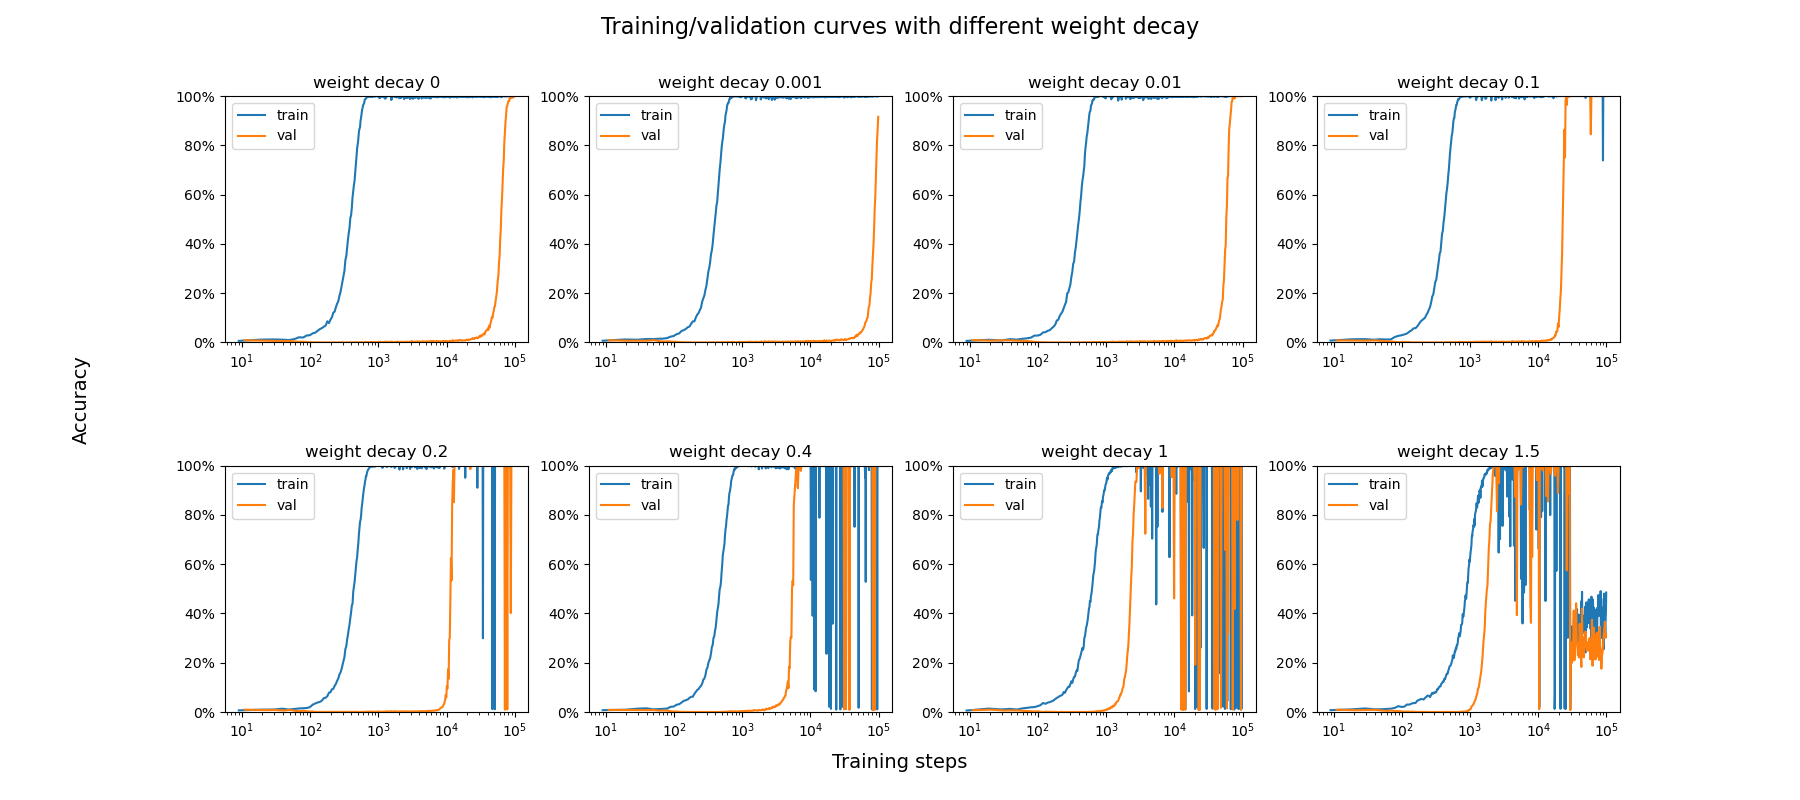
\includegraphics[width=0.9\textwidth]{fig/weight_decay/weight_decay.png}
    \caption{Grokking phenomenon for different weight decay}
    \label{fig:different weight_decay}
\end{figure}

In \cref{fig:different_settings}, the AdamW in baseline can do well when $\alpha = 33\%$, but the AdamW with 0.1x baseline learning rate performs poorly even when alpha is 60\%,which means small learning rate may cause slow training.However,big learning rate may not necessarily lead to fast training,which can be seen from the comparison between SGD in baseline(weight decay=0) and SGD with 10x baseline learning rate.Additionally,removing dropout has little impact on AdamW, but adding weight decay makes SGD's training even worse,which are all the characteristics of methods themselves.
As for the comparison between methods, under the same learning rate and dropout settings, AdamW is the best and SGD with Nesterov acceleration is the worst. RMSprop and mini batch Adam have acceptable performance when alpha is greater than 50\%, while full batch Adam needs to exceed 70\% to reach the same level.
In \cref{fig:different weight_decay},we select a column of gradually increasing weight decay values and train them on the transformer model using AdamW. As the weight decay value gradually increases, the number of training steps required to reach validation accuracy close to 100\% decreases, and the grokking phenomenon becomes less obvious. However, it is worth noting that when the weight decay value exceeds 0.2, there are occasional "rollback" phenomena in training accuracy and validation accuracy on certain training steps, which occur more frequently as the weight decay value increases. When the weight decay value is 1.5 and the training steps exceed 3e4, accuracy cannot even be restored. The reason is worth further exploration, but at least it tells us that the selection of training steps does not need to be too large.